\documentclass[11pt,a4paper]{article}
\usepackage[utf8]{inputenc}
\usepackage[T1]{fontenc}
\usepackage{lmodern}
\usepackage{geometry}
\geometry{margin=2.5cm}
\usepackage{graphicx}
% Packages for code listings
\usepackage{listings}
\usepackage{xcolor}
% Packages for drawing figures
\usepackage{tikz}
\usetikzlibrary{arrows.meta, positioning, shapes.geometric}
\usepackage{hyperref}

% Define colors for code listings
\definecolor{codegreen}{rgb}{0,0.6,0}
\definecolor{codegray}{rgb}{0.5,0.5,0.5}
\definecolor{codepurple}{rgb}{0.58,0,0.82}
\definecolor{backcolour}{rgb}{0.95,0.95,0.92}

% Setup code listing style
\lstdefinestyle{mystyle}{
    backgroundcolor=\color{backcolour},
    commentstyle=\color{codegreen},
    keywordstyle=\color{magenta},
    numberstyle=\tiny\color{codegray},
    stringstyle=\color{codepurple},
    basicstyle=\ttfamily\footnotesize,
    breakatwhitespace=false,
    breaklines=true,
    captionpos=b,
    keepspaces=true,
    numbers=left,
    numbersep=5pt,
    showspaces=false,
    showstringspaces=false,
    showtabs=false,
    tabsize=4,
    frame=single
}
\lstset{style=mystyle}

\title{Practical 3: MPI File Transfer Report}
\author{Le Quy Ton \\ 23BI14425}
\date{\today}

\begin{document}
\maketitle

\section{Task Overview}
The objective of this practical work is to upgrade a previously implemented TCP file transfer system into a system utilizing the Message Passing Interface (MPI) standard. The implementation is done in Python using the \texttt{mpi4py} library.

\section{Choice of MPI Implementation}
I chose \texttt{mpi4py} (Python bindings for MPI) for the following reasons:
\begin{itemize}
    \item \textbf{Ease of Use:} Python allows for rapid development and simpler handling of file I/O and string manipulations compared to C/C++.
    
    \item \textbf{Direct Mapping to MPI Standard:} \texttt{mpi4py} provides a close mapping to standard MPI primitives (e.g., \texttt{MPI\_Send}, \texttt{MPI\_Recv}, \texttt{MPI\_Probe}), ensuring the design principles remain true to MPI concepts.
    
    \item \textbf{Ecosystem Integration:} It integrates seamlessly with the broader Python scientific ecosystem if further data processing is needed later.
\end{itemize}

\section{System Organization}
The system is organized in a centralized "star" topology, adopting a Client-Server model tailored for MPI ranks.

\begin{itemize}
    \item \textbf{Rank 0 (The Receiver/Server):} This process acts as the central repository. It determines the number of potential senders and enters a listening state, ready to receive files from any other rank.
    
    \item \textbf{Rank 1 to N (The Senders/Clients):} These processes identify their assigned file from command-line arguments, initiate connection to Rank 0, and push their data.
\end{itemize}

Figure \ref{fig:system_org} illustrates this organization where multiple sender ranks transmit data to the single receiver rank.

\begin{figure}[ht]
    \centering
    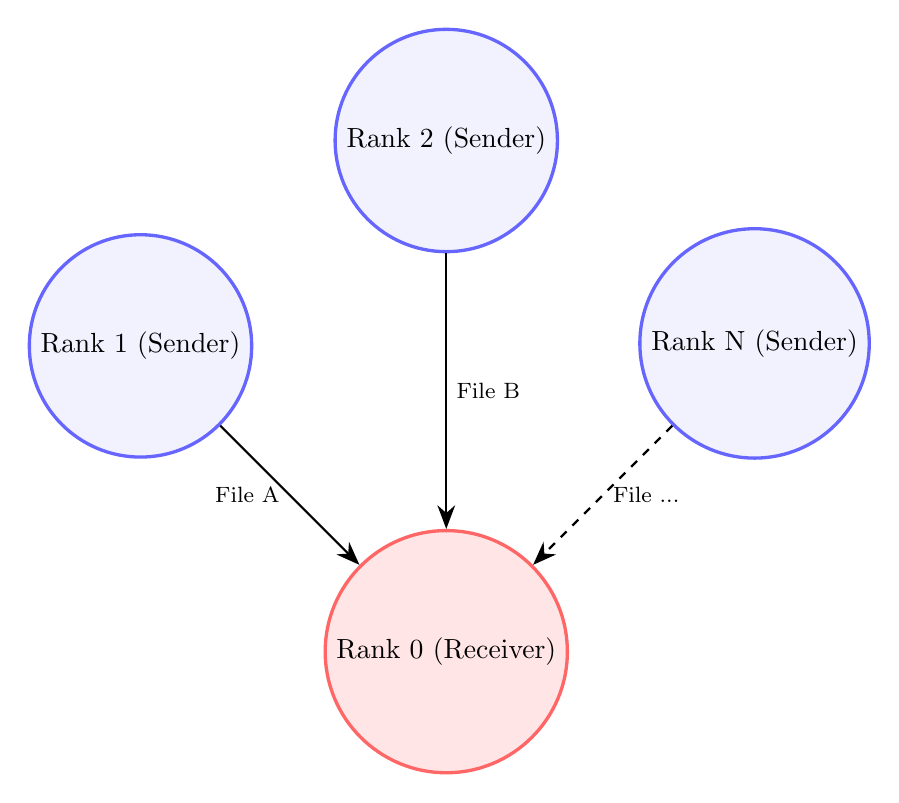
\begin{tikzpicture}[
        node distance=2.5cm,
        proc/.style={circle, draw=blue!60, fill=blue!5, very thick, minimum size=1.5cm},
        arrow/.style={->, -{Stealth[length=3mm]}, thick}
    ]
        % Nodes
        \node[proc, fill=red!10, draw=red!60] (R0) {Rank 0 (Receiver)};
        \node[proc, above left=of R0] (R1) {Rank 1 (Sender)};
        \node[proc, above=of R0, yshift=1cm] (R2) {Rank 2 (Sender)};
        \node[proc, above right=of R0] (R3) {Rank N (Sender)};

        % Arrows
        \draw[arrow] (R1) -- node[midway, left, font=\footnotesize] {File A} (R0);
        \draw[arrow] (R2) -- node[midway, right, font=\footnotesize] {File B} (R0);
        \draw[arrow, dashed] (R3) -- node[midway, right, font=\footnotesize] {File ...} (R0);

    \end{tikzpicture}
    \caption{System Organization: Multiple Senders pushing files to Rank 0.}
    \label{fig:system_org}
\end{figure}

\section{Service Design and Protocol}
The file transfer service is designed around a strictly ordered, metadata-first protocol to ensure robust transmission. To handle potentially large files, data is transmitted in fixed-size chunks (4096 bytes).

The communication sequence between a Sender (Rank $i$) and the Receiver (Rank 0) is as follows:
\begin{enumerate}
    \item \textbf{Metadata Header:} The sender first transmits essential file metadata: filename length, filename string, and total file size.
    
    \item \textbf{Data Payload:} The file content is read in chunks and sent sequentially using a specific \texttt{TAG\_DATA}.
    
    \item \textbf{Completion Signal:} Once all data is sent, a final zero-byte message with \texttt{TAG\_DONE} is sent to signal the end of the transfer.
\end{enumerate}

Figure \ref{fig:sequence} depicts the timeline of messages exchanged during a single file transfer session.

\begin{figure}[ht]
    \centering
    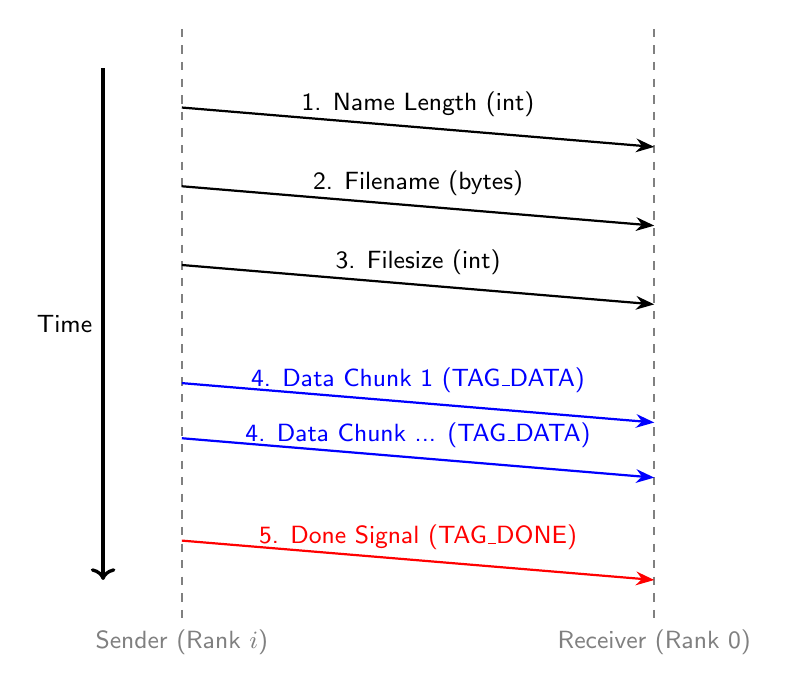
\begin{tikzpicture}[
        yscale=-1, % Reverse y-axis for timeline view
        every node/.style={font=\sffamily\small},
        msg/.style={-Stealth, thick},
        timeline/.style={dashed, thick, gray}
    ]
        % Define coordinates
        \coordinate (S_top) at (0,0); \coordinate (S_bottom) at (0,7.5);
        \coordinate (R_top) at (6,0); \coordinate (R_bottom) at (6,7.5);

        % Draw Timelines
        \draw[timeline] (S_top) -- (S_bottom) node[below] {Sender (Rank $i$)};
        \draw[timeline] (R_top) -- (R_bottom) node[below] {Receiver (Rank 0)};

        % Messages
        \draw[msg] (0, 1.0) -- (6, 1.5) node[midway, above] {1. Name Length (int)};
        \draw[msg] (0, 2.0) -- (6, 2.5) node[midway, above] {2. Filename (bytes)};
        \draw[msg] (0, 3.0) -- (6, 3.5) node[midway, above] {3. Filesize (int)};

        \draw[msg, blue] (0, 4.5) -- (6, 5.0) node[midway, above] {4. Data Chunk 1 (TAG\_DATA)};
        \draw[msg, blue] (0, 5.2) -- (6, 5.7) node[midway, above] {4. Data Chunk ... (TAG\_DATA)};

        \draw[msg, red] (0, 6.5) -- (6, 7.0) node[midway, above] {5. Done Signal (TAG\_DONE)};

        % Time arrow
        \draw[->, very thick] (-1, 0.5) -- (-1, 7) node[midway, left] {Time};

    \end{tikzpicture}
    \caption{Sequence Diagram of the MPI File Transfer Protocol.}
    \label{fig:sequence}
\end{figure}

\section{Implementation Details}
The implementation uses standard blocking MPI calls. A key aspect of the receiver implementation is the use of \texttt{comm.Probe()}. Since data is arriving in unknown chunk sizes (up to 4096 bytes) and the stream is terminated by a specific tag, the receiver probes incoming messages to determine their size and tag before allocating a buffer and committing to a receive operation.

Below are the critical code snippets illustrating the core logic.

\subsection{Sender Implementation Snippet}
The sender reads the file in chunks and uses the uppercase \texttt{comm.Send} for efficient transmission of raw byte buffers.

\begin{lstlisting}[language=Python, caption=Core sender loop transmitting file data.]
# (Inside sender function)
# send data in chunks
with open(filepath, 'rb') as f:
    sent = 0
    while sent < filesize:
        chunk = f.read(CHUNK)
        if not chunk:
            break
        # send raw bytes
        comm.Send([chunk, MPI.BYTE], dest=dest, tag=TAG_DATA)
        sent += len(chunk)
# notify done
comm.send(True, dest=dest, tag=TAG_DONE)
print(f"[rank {rank}][SENDER] Sent '{fname}' ({filesize} bytes) to rank {dest}.", flush=True)
\end{lstlisting}

\subsection{Receiver Implementation Snippet}
The receiver loops until the total expected bytes are received. It uses \texttt{Probe} to dynamically handle incoming data chunks or the completion signal.

\begin{lstlisting}[language=Python, caption=Receiver loop using Probe to handle incoming chunks.]
# (Inside receiver function loop)
received = 0
with open(out_name, 'wb') as out:
    while received < filesize:
        # Probe for next incoming message
        status = MPI.Status()
        comm.Probe(source=expected_from, tag=MPI.ANY_TAG, status=status)
        t = status.Get_tag()
        if t == TAG_DATA:
            count = status.Get_count(MPI.BYTE)
            buf = bytearray(count)
            comm.Recv([buf, MPI.BYTE], source=expected_from, tag=TAG_DATA, status=status)
            out.write(buf)
            received += count
        elif t == TAG_DONE:
            # consume the done message and break
            _ = comm.recv(source=expected_from, tag=TAG_DONE)
            break
        else:
            # unexpected tag; try to consume and continue
            comm.recv(source=expected_from, tag=t)
\end{lstlisting}

\section{How to Run}
The program requires an MPI runtime (e.g., OpenMPI or MPICH) and the \texttt{mpi4py} library. Rank 0 is automatically designated as the receiver.

To transfer two files using 3 processes (1 receiver, 2 senders):
\begin{verbatim}
mpirun -np 3 python3 mpi_transfer.py send file1.txt file2.txt
\end{verbatim}

Rank 1 will send \texttt{file1.txt}, and Rank 2 will send \texttt{file2.txt}. The receiver will save them with prefixes indicating their source rank.

\end{document}
